%
% het_node_doc.tex
%
% Copyright (C) 2015, Achim Lösch <achim.loesch@upb.de>, Christoph Knorr <cknorr@mail.uni-paderborn.de>
% All rights reserved.
%
% This documentation may be modified and distributed under the terms
% of the BSD license. See the LICENSE file for details.
%
% encoding: UTF-8
% tab size: 4
%
% author: Achim Lösch (achim.loesch@upb.de)
% created: 7/20/14
% version: 0.5.8 - change project name to ampehre
%

\documentclass[a4paper,10pt]{article}

\usepackage[english]{babel}
\usepackage[utf8]{inputenc}
\usepackage{graphicx}
\usepackage{listings}
\usepackage{framed, color}
\usepackage{colortbl}
\usepackage{amssymb}
\usepackage[markup=default]{changes}
\usepackage{hhline}
\usepackage{tabularx}
\usepackage[titletoc]{appendix}
\usepackage{pdflscape}

\graphicspath{{./figures/}}

\definecolor{lightgray}{rgb}{0.7,0.7,0.7}
\definecolor{codegreen}{rgb}{0,0.6,0}
\definecolor{codegray}{rgb}{0.5,0.5,0.5}
\definecolor{codepurple}{rgb}{0.58,0,0.82}
\definecolor{backcolour}{rgb}{0.95,0.95,0.92}

\lstdefinestyle{mystyle}{
	backgroundcolor=\color{backcolour},
	commentstyle=\color{codegreen},
	keywordstyle=\color{magenta},
	numberstyle=\tiny\color{codegray},
	stringstyle=\color{codepurple},
	basicstyle=\footnotesize,
	breakatwhitespace=false,
	breaklines=true,
	captionpos=b,
	keepspaces=true,
	numbers=left,
	numbersep=5pt,
	showspaces=false,
	showstringspaces=false,
	showtabs=false,
	tabsize=4
}
\lstset{language=C++,frame=shadowbox,frameround=tftf, numbers =left,captionpos=b, style=mystyle}

\definechangesauthor[name={Christoph Knorr}, color=orange]{ck}
\definechangesauthor[name={Achim Lösch}, color=blue]{al}

\begin{document}

%
% titlepage.tex
%
% Copyright (C) 2015, Achim Lösch <achim.loesch@upb.de>, Christoph Knorr <cknorr@mail.uni-paderborn.de>
% All rights reserved.
%
% This documentation may be modified and distributed under the terms
% of the BSD license. See the LICENSE file for details.
%
% encoding: UTF-8
% tab size: 4
%
% author: Achim Lösch (achim.loesch@upb.de)
% created: 7/21/14
% version: 0.5.8 - change project name to ampehre
%          0.6.0 - add ioctl for the ipmi timeout, new parameters to skip certain measurements 
%                  and to select between the full or light library. 
%

\begin{titlepage}

\begin{center}


\includegraphics[width=0.7\textwidth]{figures/ampehre_logo.png}\\[1cm]

\textit{\LARGE \textbf{A}ccurately \textbf{M}easuring \textbf{P}ower and \textbf{E}nergy for \textbf{H}eterogeneous \textbf{R}esource \textbf{E}nvironments}\\[1cm]

\textsc{\Large University of Paderborn, Germany}\\[1cm]

\newcommand{\HRule}{\rule{\linewidth}{0.5mm}} \HRule \\[0.6cm] { \huge Ampehre v0.8.0}\\[0.4cm]

\HRule\\[1cm]

\begin{minipage}{0.4\textwidth} \begin{center} \large \emph{Authors:}\\ Achim \textsc{L\"osch}\\Ahmad \textsc{El-Ali} \end{center} \end{minipage}

\vfill

{\Large \today}

\end{center}

\end{titlepage}

\tableofcontents

\clearpage
%
% project.tex
%
% Copyright (C) 2015, Achim Lösch <achim.loesch@upb.de>, Christoph Knorr <cknorr@mail.uni-paderborn.de>
% All rights reserved.
%
% This documentation may be modified and distributed under the terms
% of the BSD license. See the LICENSE file for details.
%
% encoding: UTF-8
% tab size: 4
%
% author: Achim Lösch (achim.loesch@upb.de)
% created: 7/24/14
% version: 0.5.8 - change project name to ampehre
%

\section{Project Description}
The Ampehre project is a BSD-licensed modular software framework used to sample various types of sensors embedded in integrated circuits or on circuit boards deployed to servers with a focus to heterogeneous computing.
It enables accurate measurements of power, energy, temperature, and device utilization for computing resources such as CPUs (Central Processing Unit), GPUs (Graphics Processing Unit), FPGAs (Field Programmable Gate Array), and MICs (Many Integrated Core) as well as system-wide measuring via IPMI (Intelligent Platform Management Platform).
For this, no dedicated measuring equipment such as DMMs (Digital Multimeter) is needed.
We have implemented the software in a way that the influence of the measuring procedures running as a multi-threaded CPU task has a minimum impact to the overall CPU load.
The modular design of the software facilitates the integration of new resources.
 Though it has been enabled to integrate new resources since version v0.5.1, the effort to do so is still quite high.
Accordingly, our plans for the next releases are broader improvements on the resource integration as well as an extensive project review to stabilize the code base.

Until version v0.8.0 the library used for resource measurement was \emph{libmeasurement}.
From version v1.0.0 on alternatively the PAPI library can be used to execute the measurements.
For this the wrapper library \emph{libapapi} was created to make the PAPI capabilities available through the well-known interface of \emph{libmeasurement}.
By default the tools use \emph{libmeasurement}.

\clearpage
%
% build.tex
%
% Copyright (C) 2015, Achim Lösch <achim.loesch@upb.de>, Christoph Knorr <cknorr@mail.uni-paderborn.de>
% All rights reserved.
%
% This documentation may be modified and distributed under the terms
% of the BSD license. See the LICENSE file for details.
%
% encoding: UTF-8
% tab size: 4
%
% author: Achim Lösch (achim.loesch@upb.de)
% created: 7/24/14
% version: 0.5.8 - change project name to ampehre
%

\section{Build instructions}

Required dependencies:
\begin{itemize}
    \item CMake
    \item gcc, g++
\end{itemize}

\noindent Optional dependencies:
\begin{itemize}
    \item NVML for Nvidia GPU support
    \item maxeleros for Maxeler FPGA support
    \item mpss-micmgmt for Intel Xeon Phi support
    \item cpufrequtils/cpupowerutils
    \item QT and QWT for GUI tools
\end{itemize}

\noindent Included dependencies:
\begin{itemize}
    \item PAPI
    \item cjson
\end{itemize}

\subsection{Cloning}

Clone the project to a local directory.

~

\verb+git clone --recurse-submodules https://github.com/akiml/ampehre+

~

\noindent This also clones the PAPI repository as a submodule to the \verb+papi/+ folder.

\subsection{Building}

Ampehre uses CMake as primary build system.
The Makefile is used for starting the build, installing and cleaning up.
Run \verb+make+ to start the build process into the subdirectory \verb+build/+.

The PAPI build process was not changed and is triggered from the CMake build script.
The called script can be found in the file \verb+papi/cmake_build.sh+.

Run \verb+make clean+ to clean the CMake and PAPI build folders.

Using \verb+make install+ you can install Ampehre to your system.

\subsection{Adjust build parameters}

It might be necessary to adjust certain build parameters.
Foremost you can change paths to \emph{gcc} and \emph{g++} inside the file \verb+Makefile+.
Next you can deactivate options for certain supported measurement sources at the top of the root \verb+CMakeLists.txt+.

You might have a newer version of cpufrequtils installed named cpupowerutils.
In this case adjust the linked library in \\\verb+libmeasure/cpu_intel_xeon_sandy/CMakeLists.txt+ or create a symlink to \verb+libcpupower.so+ called \verb+libcpufreq.so+ at the adequate position.
However, there is no guarantee for compatibility to newer versions.

In case the paths to optional dependencies for the NVML or Maxeler libraries can't be found, adjust the search paths in the \emph{find external libraries} section of the root CMake file \verb+CMakeLists.txt+.

Note that it is most certainly necessary to call \verb+make clean+ after changing build parameters to remove the CMake cache and generated Makefiles.

\subsection{Linux Kernel Modules}

The \emph{driver\_measure} module offers access to mainboard power readings through DELL IDRAC7 IPMI messages.
To build and install the \emph{driver\_measure} module run \verb+make+ and \verb+make install+ in \verb+driver/+.
There are folders with two versions: the module in \verb+driver+ offers IPMI and MSR measurements, while the module in \verb+driver_ipmi+ only supports IPMI.
The old \emph{libmeasurement} requires the module in \verb+driver+.

The \emph{amsr} module offers access to MSR values used to read energy, temperature and frequency values for Intel CPUs.
It is a modified version of the original \emph{msr} kernel module, extended with whitelisting of available registers.
The \emph{amsr} device nodes can be made available to normal users since only whitelisted registers are accessible.
To add registers to the whitelist modify the arrays at the top of the \verb+amsr.c+ file and rebuild.
To build the \emph{amsr} module run \verb+make+.
Note: \emph{msr\_safe} is a similar kernel module supported by the PAPI rapl component.

For both modules, make sure that the respective device files are accessible to users.
Adjust accessibility using \emph{chmod}.



\clearpage
%%
% overview.tex
%
% Copyright (C) 2015, Achim Lösch <achim.loesch@upb.de>, Christoph Knorr <cknorr@mail.uni-paderborn.de>
% All rights reserved.
%
% This documentation may be modified and distributed under the terms
% of the BSD license. See the LICENSE file for details.
%
% encoding: UTF-8
% tab size: 4
%
% author: Achim Lösch (achim.loesch@upb.de)
% created: 7/24/14
% version: 0.5.8 - change project name to ampehre
%

\section{Component Overview}
The Ampehre project consists of several libraries and executables to provide an easy extendable modular software framework to measure various physical values such as power, energy, and temperature of integrated circuits and boards of heterogeneous high-performance computers. Figure \ref{fig:ampehre_overview} presents an overview of project components and their location in the repository's directory structure. In the following paragraph we briefly describe each component.

\begin{figure}
\begin{center}
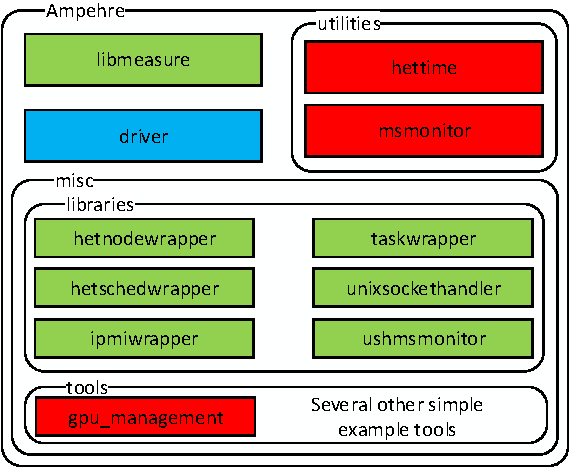
\includegraphics[width=0.8\textwidth]{ampehre_project_overview} 
\caption{Ampehre project overview showing the directory structure (rounded rectangles) and different components (green: libraries, red: executables, blue: linux kernel module).}
\label{fig:ampehre_overview}
\end{center}
\end{figure}

\begin{description}
	\item[libmeasure:] Contains the main components of the ampehre project. The measuring library consists of several modules compiled to seperate shared objects used to measure physical values such as power, energy, temperature, and utilization of resources deployed to a single heterogeneous compute node. Each of these modules implements the measuring functionality related to one of the measured resources. We describe the structure of the modules in detail in section \ref{sec:SoftwareArchitecture}. 
% 	Currently the library is made of the following resource specific modules:
% 	\begin{itemize}
% 	\item \textbf{cpu\_intel\_xeon\_sandy}: Energy, power, temperature, frequency, utilization and memory occupancy measurements.
% 	\item \textbf{fpga\_maxeler\_max3a}: Energy, power, temperature and utilization measurements.
% 	\item \textbf{gpu\_nvidia\_tesla\_kepler}: Energy, power, temperature, frequency, utilization and memory occupancy measurements.
% 	\item \textbf{mic\_intel\_knc}: Energy, power, temperature, frequency, utilization and memory occupancy measurements.
% 	\item \textbf{sys\_dell\_idrac7}: Energy, power and temperature measurements of the system board and energy and power of the complete system. 
% 	\end{itemize}
% 	
	\item[\textbf{hettime:}] Allows us to measure the energy consumption, average power dissipation, maximum device temperature, and the CPU utilization of all supported resources while executing a binary given via command line. For this the utility uses the functionality provided by the libmeasure. The results are printed to the shell or stored as a csv.
	
	\item[\textbf{msmonitor:}] Is a live monitoring tool which uses our libmeasure to retrieve current measurement values for power consumption, temperature, clock frequencies, utilization and the sum of allocated memory of the different resources. All values are shown in a Qt4-based user interface using the qwt library for plotting curves. This tool is also quite useful for debugging programms with unexpected "energy behavior".
	
	\item[driver:] Contains a dynamically loadable kernel module. Our kernel module reads CPU MSRs (Model Specific Register), memory and swap occupancy, and the CPU utilization values provided by the Linux OS. Furthermore, the kernel module allows sending IPMI (Intelligent Platform Management Interface) requests to the BMC (Baseboard Management Controller). The driver functions are available through the character device \texttt{/dev/measure}.
	
	\item[ipmiwrapper:] Provides functions to get the measured values of specific sensors via IPMI and also for DELL-specific IPMI requests. Internally, this library uses the \texttt{/dev/measure} device to send raw IPMI messages to the BMC and converts the response messages to double or integer values which are processed by the libmeasure. 
	
	\item[\textbf{gpu\_management:}] Is used to set the GPU memory and core clock frequenices and to enable or disable the Nvidia driver's persistence mode. The NVML (Nvidia Management Library) is required by the tool and is usually installed alongside Nvidia driver and CUDA packages. You can find the corresponding header file in the Nvidia GPU Deployment Kit.
	
	\item[\textbf{taskwrapper}:] Provides an interface to perform multiple energy measurements simultaneously. Since energy is the integral of power over time, we have to sample the power dissipation measured by device sensors periodically to compute a discrete approximation of the actual energy consumption. If multiple threads would perform different measurements, the same resources would be sampled concurrently, which has bad influence to the CPU load. The taskwrapper provides a simple mechanism to prevent concurrent measurements, by reading every sensor once every few milliseconds and calculating the energy consumed in the meantime individually for each registered thread. This feature can be useful, if you have one thread executing a GPU kernel while another thread is processing an FPGA kernel. This feature is less helpful, if you measure the energy consumption of multiple tasks running on the CPU simultaneously, as the energy consumption induced by one thread will invalidate the measurement result of the other task (and vice versa, of course).
	
	\item[\textbf{hetnodewrapper}:] Provides a simplified interface to the libmeasure which allows multiple measurements. Only one measurement is instantiated in the libmeasure and the values of this measurement are sampled by the hetnodewrapper at the beginning and end of every measurement. The subtractions of the particular final and first measurements are the actual result used for returned measurements. The library retrieves runtime, energy, and utilization measurements for CPU, GPU, FPGA, and the mainboard respectively power supply.
	
	\item[\textbf{hetschedwrapper}:] Uses the taskwrapper for measurements providing a more abstract interface. The wrapper is used by an external project not embedded in this repository.
	
	\item[\textbf{unixsockethandler:}] Implements a communication layer for client-server IPC, based on Unix sockets with the advantage of a simple interface hiding the system calls.
	
	\item[\textbf{ushmsmonitor:}] Is a library enhancing the general-purpose Unix socket-based IPC implementation of the unixsockethandler library. Our msmonitor monitoring utility uses the ushmsmonitor library as a server listening to a Unix socket. A client such as hettime must implement the counterpart. The clients can transmit start and stop signals to the server. Accordingly, servers are able to perform any activity after receiving these signals. For instance, out msmonitor tool shows start and stop markers on the qwt plots as well as the client's PID sending the corresponding signals.
\end{description}

Additionally, the \texttt{/misc/tools} directory contains several simple example programs which use the mentioned libraries. Each executable allows us to test a specific functionality of our project. \textbf{The \texttt{example\_ms} tool shows all function calls which are necessary to perform measurements with our measuring library.}

%
% usage.tex
%
% Copyright (C) 2015, Achim Lösch <achim.loesch@upb.de>, Christoph Knorr <cknorr@mail.uni-paderborn.de>
% All rights reserved.
%
% This documentation may be modified and distributed under the terms
% of the BSD license. See the LICENSE file for details.
%
% encoding: UTF-8
% tab size: 4
%
% author: Achim Lösch (achim.loesch@upb.de)
% created: 7/24/14
% version: 0.5.8 - change project name to ampehre
%

\section{Usage}

Ampehre provides several possibilities to execute measurements.
\begin{itemize}
\item Measurement of a complete program execution
\item Integration into your own program to measure a certain section
\item Live monitoring of the system including a graphical output
\end{itemize}

\subsection{Tools}

\subsubsection{hettime}
\emph{hettime} allows to measure the execution of a newly started application similar to \emph{time}.
For this hettime starts the measurement, executes the program and waits for its completion before stopping the measurement.
hettime has several parameters to configure the measurement, but it expects at least the path to the executable.
Using \verb+-a+ you can pass arguments to the measured program.

~

\verb+hettime [OPTIONS] -e EXECUTABLE [-a ARGS]+

~

By default measurements for the modules are performed at a sampling rate of 100 ms.
To adjust the sampling rate use the following parameters in ms:

~

\verb+-c SAMPLE_CPU+

\verb+-g SAMPLE_GPU+

\verb+-f SAMPLE_FPGA+

\verb+-m SAMPLE_MIC+

\verb+-s SAMPLE_SYS+

~

By default hettime uses the libmeasurement library for measurment.
To start hettime with the libapapi library use the \verb+LD_PRELOAD+ environment variable.

~

\verb+LD_PRELOAD=/path/to/libms_common_apapi.so hettime+

~

This allows to use additional configuration of the APAPI library.

\subsubsection{msmonitor}

To do a live monitoring of your system you can use the msmonitor gui tool.

\subsubsection{msmonitor\_cs}

To use msmonitor remotely start the msmonitor server program on the host you want to monitor, the default port is 2900:

\verb+msmonitor_server [-p PORT]+

Now you can start the client on a different host to receive the monitored data:

\verb+msmonitor_client+

In the settings menu you can define the target address and port to connect to the monitored server.

\subsection{Program integration}

To integrate the measurement tool in your own program you need to include the \verb+ms_measurement.h+ header file and link against the \verb+libms_common.so+ library.
Now you can make use of the measurement library to measure a certain section of you program.
The following listing shows the necessary steps to execute a measurement.

\begin{lstlisting}
// initialize the measurement library using the default parameters
MS_VERSION version = { .major = MS_MAJOR_VERSION,
                       .minor = MS_MINOR_VERSION,
                       .revision = MS_REVISION_VERSION };
MS_SYSTEM *ms = ms_init(&version, CPU_GOVERNOR_ONDEMAND,
                      2000000, 2500000, GPU_FREQUENCY_CUR, 
                      IPMI_SET_TIMEOUT, SKIP_PERIODIC,
                      VARIANT_FULL);

// allocate the data structure for one measurement
MS_LIST *m1 = ms_alloc_measurement(ms);

// Set timer for m1
// Measurements perform every (10ms/30ms)
ms_set_timer(m1, CPU,    0, 10000000, 10);
ms_set_timer(m1, GPU,    0, 10000000, 10);
ms_set_timer(m1, FPGA,   0, 30000000, 10);
ms_set_timer(m1, SYSTEM, 0, 30000000, 10);
ms_set_timer(m1, MIC,    0, 30000000, 10);

// setup the m1 data structure for the next measurement
ms_init_measurement(ms, m1, CPU | GPU | FPGA | SYSTEM | MIC);

// measure the section you want to analyze
ms_start_measurement(ms);

do_something();

ms_stop_measurement(ms);
ms_join_measurement(ms);
ms_fini_measurement(ms);

// now you can look at the results

// destroy the measurement data structure
ms_free_measurement(m1);

// finally shutdown the measurement library
ms_fini(ms);
\end{lstlisting}

To analyze the measurement results use the methods in the respective module headers.

\begin{lstlisting}
// method for dram energy consumption
// defined in the ms_cpu_intel_xeon_sandy.h header
printf("consumed energy of cpu 1 dram bank : %.2lf mWs\n",
           cpu_energy_total_dram(m, 1));
\end{lstlisting}

\subsection{APAPI configuration}

On invocation libapapi reads certain environment variables for configuration.
This might be especially handy when using hettime with libapapi.
The detailed file formats are described in appendix \ref{appendixapapi}.

\begin{itemize}
\item \verb+APAPI_CMPLIST+ allows to define which components are measured.
The default is \verb+rapl:nvml:maxeler:micknc:ipmi+
\item \verb+APAPI_EVENTLIST+ allows to define the list of events per component that are measured.
The default list \verb+default_eventlist.txt+ is included.
\item \verb+APAPI_EVENTOPS+ allows to define how the events are processed.
This is only needed when adding new events.
The default list \verb+default_eventops.txt+ is included.
\end{itemize}



\clearpage
\section{Extend measurement capabilities}

To add additional indicators you need to modify several files:

\begin{itemize}
\item PAPI component
\item libapapi event definitions
\item libapapi value copying
\item libmeasurement data structures and methods
\end{itemize}

\subsection{PAPI component}
The PAPI library supports extension by defining a new component.
The components can be found in the \verb+papi/src/components+ directory and every component has its own folder.
If you want to create a completely new component you can find an example component in the \verb+example+ folder.
Every component creates an internal list of available events on initialization in \verb+_example_init_component+.
\verb+_example_update_control_state+ is called to maintain a struct that contains the chosen events.
If the read method \verb+_example_read+ is called the values of chosen events need to be read and copied to the output array.
In all of this steps the different events need to be handled and modified in case of extension, however available components contain additional support methods.

If a new component is created it needs to be added to the list of compiled components \verb+--with-components+ in the build script \verb+papi/cmake_build.sh+.

\subsection{libapapi event definitions}

Once the component is available in PAPI the event definitions for libapapi must be adjusted.
The detailed file formats are described in appendix \ref{appendixapapi}.

The file defined in the environment variable \verb+APAPI_EVENTLIST+ contains the list of events to be considered if a component is activated.
Simply add the new events to the list similar to the default file.
Since the specified file will override the default file you also need to copy the desired events from the default file into the specified eventlist file.

The file defined in the environment variable \verb+APAPI_EVENTOPS+ contains a list of parameters that specifiy how to handle event values.
Accumulating values are treated differently.
Add a new entry per event according to the specifications in the appendix.
Your specified file will be merged with the default definitions so no copying of default definitions is necessary, except to override a default definition.

Finally, to activate the component you need to declare the list of used components in the \verb+APAPI_CMPLIST+ environment variable.

\subsection{libmeasurement data structures and methods}

For every libmeasurement component exists a struct containing the desired variables and the accessing methods.

\subsection{libapapi value copying}

To copy the measured event values to the libmeasurement structs the \verb+libms_common_apapi+ wrapper copies the values from the internal PAPI arrays into the target data structures.
To minimize the overhead of event traversing a list of mappings between the PAPI arrays and the libmeasurement structs are created in the method \verb+__create_mapper+.
Follow the pattern of the existing entries of checking the current component and existence of the event and finally defining the four entries for the mapping:

\begin{itemize}
\item \verb+source+ -- pointer to the PAPI array entry
\item \verb+destination+ -- pointer to the struct variable
\item \verb+type+ -- type conversion specifier
\item \verb+factor+ -- factor to convert value to the destination prefix
\end{itemize}

For struct variables that only need to be changed at the end of the measurement, check the \verb+last_measurement+ variable.


\clearpage
%%
% hardware.tex
%
% Copyright (C) 2015, Achim Lösch <achim.loesch@upb.de>, Christoph Knorr <cknorr@mail.uni-paderborn.de>
% All rights reserved.
%
% This documentation may be modified and distributed under the terms
% of the BSD license. See the LICENSE file for details.
%
% encoding: UTF-8
% tab size: 4
%
% author: Achim Lösch (achim.loesch@upb.de)
% created: 7/24/14
% version: 0.5.8 - change project name to ampehre
%

\section{Hardware Requirements}
\label{sec:hardware}

The hardware requirements mentioned in this section are related to the resource-specific modules. For instance, if your GPU is manufactured by AMD, you cannot use our module, as the GPU module only works with Nvidia Tesla GPUs. Anyway, you are still able to use our measuring framework by disabling the GPU module (explained in Section \ref{sec:BuildInstallInstructions}).

\subsection{System}

\begin{itemize}
	\item We obtain all system-related measurements via IPMI (Intelligent Platform Management Interface) utilizing a Linux kernel module accessible via the device file system entry \texttt{/dev/measure}.
	\item With IPMI we are able to get data from thermal and power sensors of both the motherboard (systemboard) and the power supply.
	\item Our server is a \textit{Dell Poweredge T620}. Hence, in order to read some non-documented DELL features/sensors via IPMI, we implemented an additional wrapper library which composes raw IPMI messages for message exchanging with the BMC.
	\item Therefore, we guess that our measurement library can only work on \textbf{Dell} systems including \textbf{iDRAC 7} (and iDRAC 8?) BMCs.
	\item We compile the source code to a dynamically loadable module. The system module is named \texttt{libms\_sys\_dell\_idrac7.so}.
\end{itemize}

\subsection{CPU}

\begin{itemize}
	\item Most energy and thermal sensor data are stored in MSRs (Model Specific Registers) of the Intel RAPL (Running Average Power Limit) interface. We read the MSRs via our kernel module \texttt{/dev/measure}.
	\item The module is also used to collect some CPU utilization values.
	\item Additionally, we are able to set the CPU governor and other values such as minimum and maximum core frequencies via the GNU library \texttt{libcpufreq}.
	\item We deployed \textit{two Intel Xeon E5-2609 v2} CPUs (microarchitecture: Ivy Bridge) to our server.
	\item As our library samples CPU registers which are model-specific, you can use our library only on systems with compatible CPUs. We guess that \textbf{Intel} CPUs with \textbf{Sandy Bridge}, \textbf{Ivy Bridge}, or \textbf{Haswell} microarchitectures should work well, if they \textbf{don't have an integrated graphics processing unit}. Integrated graphics are often available for consumer products such as the Core i3/i5/i7-processors.
	\item We compile the source code to a dynamically loadable module. The CPU module is named \texttt{libms\_cpu\_intel\_xeon\_sandy.so}.
\end{itemize}

\subsection{GPU}

\begin{itemize}
	\item Measured values are retrieved by calling functions of the NVML (Nvidia Management Library).
	\item We deployed a \textit{Nvidia Tesla K20c} to our system.
	\item All \textbf{Nvidia Tesla} GPUs with \textbf{Kepler} microarchitecture are supported (GK104, GK110, and GK210).
	\item We compile the source code to a dynamically loadable module. The GPU module is named \texttt{libms\_gpu\_nvidia\_tesla\_kepler.so}.
\end{itemize}

\subsection{FPGA}

\begin{itemize}
	\item We utilize the MaxelerOS library to obtain power, temperature, and utilization.
	\item We deployed a \textit{Maxeler Vectis} FPGA card to our system.
	\item Currently, our library only supports \textbf{Maxeler Vectis} (MAX3A) FPGA cards.
	\item We compile the source code to a dynamically loadable module. The FPGA module is named \texttt{libms\_fpga\_maxeler\_max3a.so}.
\end{itemize}

\subsection{MIC}

\begin{itemize}
	\item We use Intel's \texttt{libmicmgmt} MIC management library to obtain the measurements.
	\item We deployed a passively cooled \textit{Intel Xeon Phi 31S1P}.
	\item All \textbf{Intel Xeon Phi} with \textbf{Knights Corner} (KNC) architecture should work well with the library.
	\item We compile the source code to a dynamically loadable module. The MIC module is named \texttt{libms\_mic\_intel\_knc.so}.
\end{itemize}

\clearpage

\begin{appendices}
\appendixpage
\section{libapapi definition file specification}
\label{appendixapapi}

\subsection{eventlist file}

Every line is interpreted as one event name.
Lines starting with '\#' are ignored.
Empty lines are ignored.

Example:

\begin{verbatim}
# rapl
rapl:::PACKAGE_ENERGY:PACKAGE0
rapl:::PACKAGE_ENERGY:PACKAGE1
rapl:::DRAM_ENERGY:PACKAGE0
rapl:::DRAM_ENERGY:PACKAGE1
\end{verbatim}

If the \verb+APAPI_EVENTLIST+ environment variable is defined and the rapl component is active, only the four specified events are measured.


\subsection{eventops file}

Every line is interpreted as one event definition.
Lines starting with '\#' are ignored.
Empty lines are ignored.
One definition consists of several fields delimited by a ','.
Fields should not contain unnecessary whitespace.
One definition consists of the following fields:

\begin{itemize}

\item event name
\item operation to use to compute value1 from value0 (last two values for value0 are called sample1 (last) and sample0 (previous))

    \begin{itemize}
    \item \verb+APAPI_OP1_SAMPLE_DIFF+
        \begin{itemize}
        \item value1 = sample1 - sample0
        \end{itemize}
    \item \verb+APAPI_OP1_SAMPLE1_MUL_DIFF_TIME+
        \begin{itemize}
        \item value1 = sample1 * (time1 - time0)
        \end{itemize}
    \item \verb+APAPI_OP1_AVG_SAMPLE_MUL_DIFF_TIME+
        \begin{itemize}
        \item    value1 = (sample0 + sample1) / 2.0 * (time1 - time0)
        \end{itemize}
    \item \verb+APAPI_OP1_DIV_DIFF_TIME+
        \begin{itemize}
        \item    value1 = sample1 / (time1 - time0)
        \end{itemize}
    \end{itemize}
\item statistics to compute for value0, single term or '|' delimited list of terms:
    \begin{itemize}
    \item \verb+APAPI_STAT_NO+ - no statistics
    \item \verb+APAPI_STAT_MIN+
    \item \verb+APAPI_STAT_MAX+
    \item \verb+APAPI_STAT_AVG+
    \item \verb+APAPI_STAT_ACC+
    \item \verb+APAPI_STAT_ALL+
    \end{itemize}
\item statistics to compute for value1
\item maximal raw counter value or 0 if counter is not accumulating
\item name for type of value0
\item unit for value0
\item factor to use for value0
\item name for type of value1
\item unit for value1
\item factor to use for value1
\end{itemize}

Example:

\begin{verbatim}
# this event is an accumulating event
# the maximal raw counter value is not zero
rapl:::PP0_ENERGY:PACKAGE1,APAPI_OP1_DIV_DIFF_TIME,APAPI_STAT_ACC,
APAPI_STAT_MIN|APAPI_STAT_MAX|APAPI_STAT_AVG,0x7fffffff8000,
energy,Ws,2147483648.0,power,W,2.147483648

# this event is not-accumulating
# the maximal raw counter value is zero
rapl:::THERM_STATUS:PACKAGE0:CPU0,APAPI_OP1_NOP,
APAPI_STAT_MIN|APAPI_STAT_MAX|APAPI_STAT_AVG,APAPI_STAT_NO,
0,temperature,C,1,-,-,1
\end{verbatim}

\emph{Note:} The line breaks in the example are due to the document layout. The original entries must not contain line breaks.

Entries from the default file and the file declared in the \verb+APAPI_EVENTOPS+ environment variable are merged.
Entries in the user specified file override entries in the default file.

%%
% appendix.tex
%
% Copyright (C) 2015, Achim Lösch <achim.loesch@upb.de>, Christoph Knorr <cknorr@mail.uni-paderborn.de>
% All rights reserved.
%
% This documentation may be modified and distributed under the terms
% of the BSD license. See the LICENSE file for details.
%
% encoding: UTF-8
% tab size: 4
%
% author: Christoph Knorr (cknorrh@mail.uni-paderborn.de)
% created: 7/27/14
% version: 0.5.8 - change project name to ampehre
%          0.5.12 - add ioctl for the ipmi timeout, new parameters to skip certain measurements 
%                   and to select between the full or light library. 
%

\section{Recommended Sampling Rates} \label{app:A}
Users must specify a sampling rate for each resource which is compiled as libmeasure module. The sampling rate defines how often measurement values are queried from the devices. Low sampling rates can produce substantial CPU load, since all the measurement threads are executed on the CPU. Hence, sampling rates have to be chosen carefully. Moreover, they have an impact on the accuracy of the measurement results and the CPU utilization. We have to find a trade-off between accuracy of the measurements and the CPU utilization which also leads to different CPU power consumption. Therefore we have methodically examined different sampling rate combinations using all five modules runnable on our heterogeneous system. \added[id=al]{We have used libmeasure in its \texttt{FULL} variant (all sensors are sampled) with high accuracy (\texttt{skip\_ms\_rate} set to \texttt{LOW}).} \added[id=al]{LOW ist zu generisch, skip wieder unklar. Wir sollten Namen ändern.} We have measured the power consumption and utilization while all resources have been in idle state. The results are shown in Figure \ref{fig:CPUUtilization} and \ref{fig:CPUPower}. Obviously, the CPU utilization and power consumption is highly dependent on specific system configurations. We hope that our results are helpful anyway.\\

Figure \ref{fig:CPUUtilization} shows the CPU utilization, sampling all sensors of all currently supported resources as specified in Section \ref{sec:hardware}. The lines indicate our recommendations to achieve utilizations below a specific thresholds. For example, the blue line indicates that the utilization induced by our measuring library loading all resource-specifc modules stays below 2 \%, if the sampling rates CPU: 40 ms, MIC: 50 ms, GPU: 40 ms, FPGA: 70 ms and System 100 ms or higher are used for the measurements.

\begin{figure}[!h]
\begin{center}
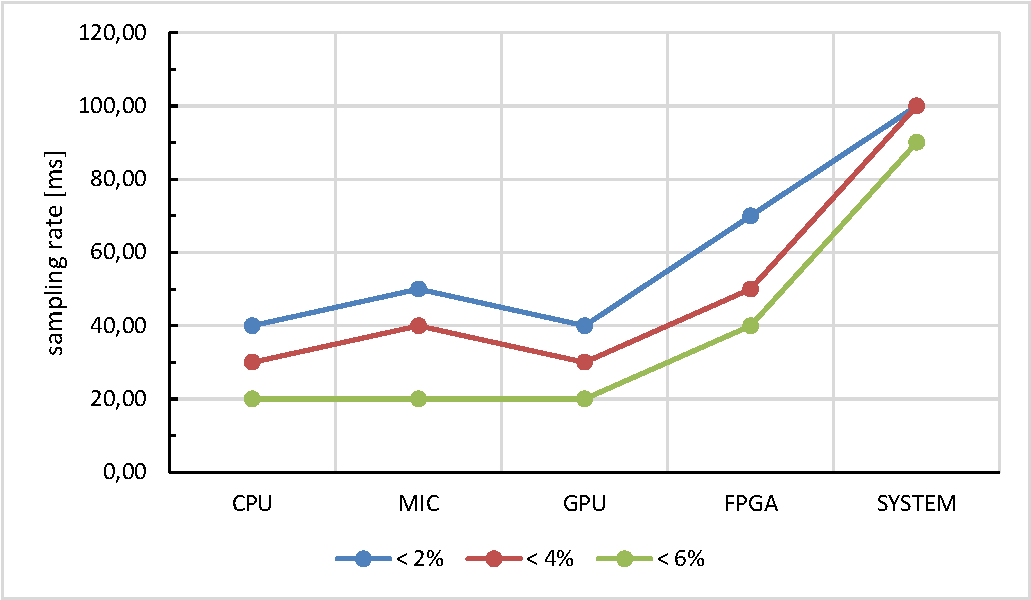
\includegraphics[width=\textwidth]{CPUUtilization} 
\caption{Libmeasure sampling rates and the resulting CPU utilization in percent. The lines indicate the lower boundaries of the sampling rates for which the CPU utilization is not higher than the corresponding threshold (2 \%, 4 \%, 6 \%).}
\label{fig:CPUUtilization}
\end{center}
\end{figure}

Figure \ref{fig:CPUPower} shows the resulting CPU power consumption induced by sampling all sensors of all currently supported resources as specified in Section \ref{sec:hardware}. Accordingly, the lines indicate what sampling rates have to be chosen to make sure that the CPU power consumption stays below specific thresholds. For example the sampling rates have to be CPU: 20 ms, MIC: 20 ms, GPU 30 ms, FPGA 40 ms, System 80 ms or higher to get a CPU power consumption of less than 18 W.\\

\begin{figure}[!h]
\begin{center}
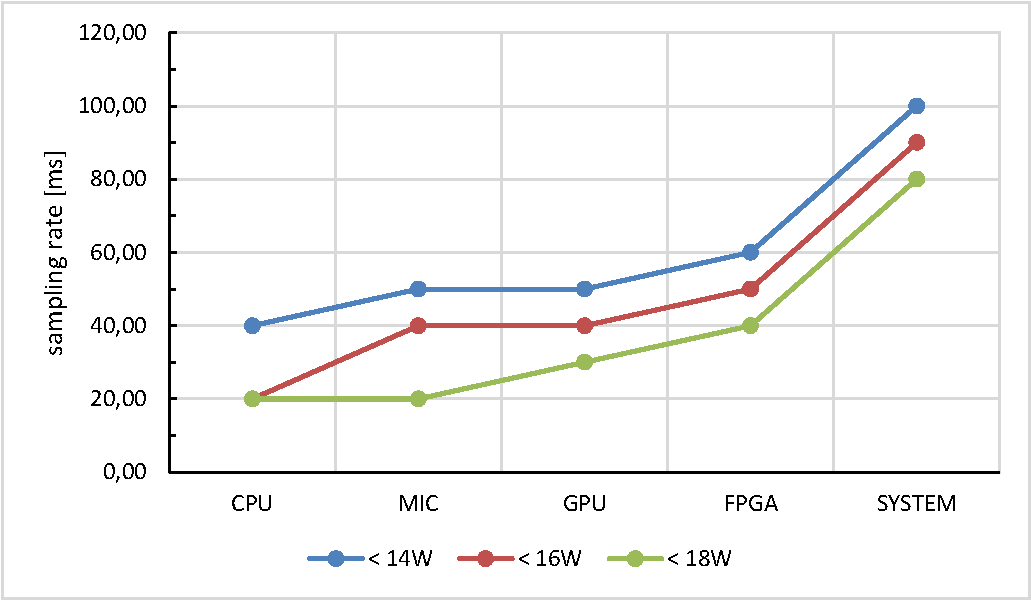
\includegraphics[width=\textwidth]{CPUPower} 
\caption{Libmeasure sampling rates and the resulting CPU Power consumption in Watt. The lines indicate the lower boundaries for which the CPU power consumption is not higher than the corresponding threshold (14 W, 16 W, 18 W).}
\label{fig:CPUPower}
\end{center}
\end{figure}

\clearpage
\section{Utility usage}
\label{app:manpage}
Each of our tools can be run with the ``-h'' option to show a help message where eyery command line option is briefly explained. The help dialog of hettime is shown in the following Listing. 
\added[id=ck]{Listing aktualisiert.}
\begin{lstlisting}[language=sh,basicstyle=\tiny,stringstyle=\color{black},keywordstyle=\color{black}]
$ hettime -h
Usage:
hettime [-h|-?|-i|-c "SAMPLE_CPU, SAMPLE_SKIP_CPU"|
		 -g "SAMPLE_GPU, SAMPLE_SKIP_GPU"|-f "SAMPLE_FPGA, SAMPLE_SKIP_FPGA"|
         -m "SAMPLE_MIC, SAMPLE_SKIP_MIC"|-s "SAMPLE_SYS, SAMPLE_SKIP_SYS"|
         -G FREQUENCY|-C GOVERNOR|-L FREQUENCY|-H FREQUENCY|-o RESULT_FILE|
         -v CSV_FILE|-u] -e EXECUTABLE [-a "ARGS"]
-c "SAMPLE_CPU,       | Sampling rate for CPU power/temp measurements in ms.
    SAMPLE_SKIP_CPU"  | Skip rate defines how many measurement points are skipped.
                      | Default: 100ms, 1. Recommended minimum: 20ms.
-g "SAMPLE_GPU,       | Sampling rate for GPU power/temp measurements in ms.
    SAMPLE_SKIP_GPU"  | Skip rate defines how many measurement points are skipped.
                      | Default: 100ms, 1. Recommended minimum: 30ms.
-f "SAMPLE_FPGA,      | Sampling rate for FPGA power/temp measurements in ms.
    SAMPLE_SKIP_FPGA" | Skip rate defines how many measurement points are skipped.
                      | Default: 100ms, 1. Recommended minimum: 50ms.
-m "SAMPLE_MIC,"      | Sampling rate for MIC power/temp measurements in ms.
    SAMPLE_SKIP_MIC"  | Skip rate defines how many measurement points are skipped.
                      | Default: 100ms, 1. Recommended minimum: 20ms.
-s "SAMPLE_SYS        | Sampling rate for system-wide power/temp measurements in ms.
    SAMPLE_SKIP_SYS"  |  Skip rate defines how many measurement points are skipped.
                      | Default: 100ms, 1. Recommended minimum: 100ms.
-S SKIP_MS_FREQ       | Skip measurement frequency defines how often certain
					  | measurements are performed.
                      | Possible settings are:
                      | high, HIGH, High
                      |    Temperature and memory information are measured
                      |    only at every 10th measuring point.
                      | low, LOW, Low
                      |    Temperature and memory information are measured
                      |    at every measuring point.
                      | Default: low.
-e EXECUTABLE         | Name of the executable. This option is mandatory.
-a "ARGS"             | Specify the arguments for executable EXECUTABLE 
					  | with this option.
                      | Note that the arguments have to be seperated by spaces.
                      | The arguments must be surrounded by quotation marks!
                      | Note that the ARGS option has to be the last
                      | in the argument list!
-G FREQUENCY          | Set a GPU frequency before the child application
					  | get started.
                      | Possible frequency settings are:
                      | min, MIN, minimum, MINIMUM
                      |    Set GPU frequency to its minimum value.
                      | max, MAX, maximum, MAXIMUM
                      |    Set GPU frequency to its maximum value.
                      | cur, CUR, current, CURRENT
                      |    Don't set GPU frequency.
                      |    Leave the current setting untouched.
                      | Default: cur.
-C GOVERNOR           | Set a CPU frequency scaling governor for the
					  | 'acpi-cpufreq' driver.
                      | Possible governors are:
                      | save, SAVE, powersave, POWERSAVE
                      |    Force CPU to use the lowest possible frequency.
                      | dmnd, DMND, ondemand, ONDEMAND
                      |    Dynamic frequency scaling. Aggresive strategy.
                      | cons, CONS, conservative, CONSERVATIVE
                      |    Dynamic frequency scaling. Conservative strategy.
                      | perf, PERF, performance, PERFORMANCE
                      |    Force CPU to use the highest possible frequency.
                      | Default: dmnd.
-L FREQUENCY          | Set the lowest permitted CPU frequency in MHz.
-H FREQUENCY          | Set the highest permitted CPU frequency in MHz.
-V LIB_VARIANT        | Defines the variant of the measuring library which is used.
                      | Possible variants are:
                      | light, LIGHT, Light
                      |    Not all possible values are measured and therefore
                      |    the CPU utilization is lower.
                      | high, HIGH, High
                      |    All values are measured.
                      | Default: full.
-o RESULT_FILE        | Save results in a file instead of printing to stdout.
-v CSV_FILE           | Save results in a CSV table file.
-u                    | Use UNIX socket handler library to communicate with
					  | msmonitor.
-i                    | Forcing FPGA to idle after measuring system initialization.
-h                    | Print this help message.
-?                    | Print this help message.

Example:
hettime -c "90, 10" -i -G min -C conservative -e /usr/bin/find -a "/usr -iname lib*"

\end{lstlisting}

\end{appendices}

\end{document}
